\documentclass[11pt,a4paper]{article}
\usepackage[margin=26mm]{geometry}
\usepackage{amsmath,amssymb,amsthm,mathtools,booktabs,microtype}
\usepackage[T1]{fontenc}
\usepackage{lmodern}
\usepackage{graphicx,array}
\usepackage[colorlinks=true,linkcolor=blue,citecolor=blue,urlcolor=blue]{hyperref}
\setlength{\emergencystretch}{2em}
\newtheorem{theorem}{Theorem}[section]
\newtheorem{proposition}[theorem]{Proposition}
\newtheorem{lemma}[theorem]{Lemma}
\newtheorem{corollary}[theorem]{Corollary}
\theoremstyle{definition}
\newtheorem{definition}[theorem]{Definition}
\theoremstyle{remark}
\newtheorem{remark}[theorem]{Remark}
\newcommand{\R}{\mathbb R}
\newcommand{\C}{\mathbb C}
\newcommand{\Z}{\mathbb Z}
\newcommand{\T}{\mathbb T}
\newcommand{\dd}{\,\mathrm d}
\newcommand{\supp}{\operatorname{supp}}
\newcommand{\Lip}{\operatorname{Lip}}
\DeclareMathOperator{\Rea}{Re}
\DeclareMathOperator{\Ima}{Im}
\title{Height Quotients of the Riemann Zero Divisor\\[3pt]
\large Central-circle limits and invisible sparse perturbations}
\author{Hayami Mathematical Research\\\small Illustrated working manuscript v0.2}
\date{18 October 2026}
\begin{document}
\maketitle
\begin{abstract}
We formulate fixed-height observations of the Riemann zero divisor on a
cylinder and on a half-twisted band. Established all-zero mod-one
 equidistribution, discrepancy and zero-density estimates give the normalized
central-circle limit and elementary support consequences. A known positive
proportion of simple critical-line zeros gives packing and closure
corollaries, without equidistribution of that subsequence. We then give a
concrete even entire product with dyadically sparse off-critical roots.
Direct estimates transfer the specified quotient limits, known smooth
prime-resonant secondary limits, and selected counting and Landau error
classes. The normalized multiplier preserves the functional equation and
pole residue but fails an ordinary Dirichlet-series condition. Prescribed
zero insertion and functional-equation nonuniqueness have substantial prior
work; our purpose is a worked synthesis with explicit quantitative controls,
not a new zero-distribution theorem or a claim of priority. Three
formula-based figures explain the construction. No result proves or refutes
the Riemann hypothesis.
\end{abstract}

\section{Question, contribution, and arithmetic inputs}

We use Riemann's entire function, with removable values understood,
\[
 \xi(s)=\tfrac12s(s-1)\pi^{-s/2}\Gamma(s/2)\zeta(s),
 \qquad \xi(1-s)=\xi(s).
\]
This is the normalization of \cite[25.4.3--25.4.4]{DLMF}; it also satisfies
$\xi(\bar s)=\overline{\xi(s)}$.
Center the critical strip by writing
\[
 \rho=\tfrac12+x_\rho+i\gamma,\qquad -\tfrac12<x_\rho<\tfrac12.
\]
A drawing that identifies heights modulo a fixed length always produces a
quotient of the ambient strip. It need not produce an invariant quotient of
its marked zero divisor. A second distinction is just as important: the raw
pushforward and its normalized finite-height probability measures have very
different behavior. We make these distinctions precise for both a cylinder
and a M\"obius band, and ask which properties of the zeros their limiting
observations can determine.

The mod-one statistics used here are prior results of Hlawka and Fujii,
recorded and developed by Ford--Zaharescu and
Ford--Soundararajan--Zaharescu \cite{FZ,FSZ}. The quotient and retraction
arguments are convenient geometric formulations of their consequences,
rather than a new zero-distribution theorem. Bui--Conrey--Young \cite{BCY}
supply the simple-critical-line proportion; our residue and closure bounds
are packing and closed-set corollaries.

Earlier close perturbations of zeta were studied by Gauthier--Zeron
\cite{GZ}.\footnote{The publisher abstract and metadata were inspected for
this historical comparison; the precise theorem comparison is to \cite{GX}.}
More precisely, Gauthier--Xarles \cite[Proposition 1 and Theorem 2]{GX}
construct symmetric prescribed-zero perturbations retaining a Riemann-type
functional equation. That work retains the
old divisor away from the prescribed set and poles/principal parts, with
strong approximation properties. Thus symmetric zero insertion itself is
not a new idea. Our product is a specific dyadic order-zero example whose
count, compact-tail and stated statistical transfers can be checked
directly; we make no claim that its individual estimates are new analytic
results. We do not obtain the strong function-value approximation of
\cite{GX}, nor infer our precise growth controls from its theorem.

A claim-targeted literature audit located no identical printed package of
this product and all the listed transfer formulas. That bounded search
result does not certify priority. The paper is presented as a worked
synthesis and an explicit diagnostic obstruction, with the comparison in
Table~\ref{tab:prior}. Functions outside the ordinary Dirichlet-series
class and converse-theorem boundaries have extensive prior literature
\cite{KMP,Burnol,Nakamura}.

\begin{table}[tbp]
\centering\small
\caption{Prior results and the limited role of the present formulation.}
\label{tab:prior}
\begin{tabular}{@{}>{\raggedright\arraybackslash}p{.24\linewidth}>{\raggedright\arraybackslash}p{.35\linewidth}>{\raggedright\arraybackslash}p{.34\linewidth}@{}}
\toprule
Prior work & Already established & Present role \\
\midrule
Hlawka; Fujii; FZ/FSZ \cite{FZ,FSZ}
& All-zero circle statistics and smooth secondary limits
& Quotient/retraction corollaries; no new distribution theorem \\
\addlinespace
Bui--Conrey--Young \cite{BCY}
& A positive proportion of simple critical-line zeros
& Elementary residue-packing and closure bounds \\
\addlinespace
Gauthier--Xarles \cite{GX}
& Symmetric zero insertion, functional equation, retained poles and approximation
& Explicit dyadic product and simultaneous transfer calculations \\
\addlinespace
Converse literature \cite{KMP,Burnol,Nakamura}
& Dirichlet-series rigidity and constructions outside that setting
& Direct real-axis obstruction for this multiplier \\
\bottomrule
\end{tabular}
\end{table}

Let $m_\rho$ be the order of a nontrivial zero and put
\[
 N(H)=\sum_{0<\Ima\rho\le H}m_\rho.
\]
Every sum over zeros in this paper includes $m_\rho$ unless distinct support
or simple zeros are explicitly specified. We use the following unconditional
inputs, with their exact scopes recorded here.

\begin{enumerate}
\item The Riemann--von Mangoldt asymptotic is
\begin{equation}\label{eq:rvm}
 N(H)=\frac{H}{2\pi}\log\frac{H}{2\pi}-\frac{H}{2\pi}+O(\log H).
\end{equation}
The count is finite in every bounded-height slab, since Riemann's entire
function $\xi$ is nonzero and its zeros are precisely the nontrivial zeta
zeros, with orders.
\item For every fixed $\alpha\ne0$, the fractional parts $\{\alpha\gamma\}$
of all nontrivial zero ordinates are uniformly distributed modulo one.
Ford--Zaharescu \cite[Introduction]{FZ} state Hlawka's unconditional theorem
and record Fujii's unconditional star-discrepancy bound
\begin{equation}\label{eq:fujii}
 D_\alpha^*(H)=O_\alpha\!\left(\frac{\log\log H}{\log H}\right).
\end{equation}
The original Hlawka and Fujii articles are identified in \cite{FZ}; our direct
source for these precisely stated consequences is that research paper.
\item If $N(\sigma,H)$ counts zeros with multiplicity, with $|\gamma|\le H$ and
$\Rea\rho\ge\sigma$, Selberg's bound as stated in
\cite[Lemma 2]{FZ} is, uniformly for $1/2\le\sigma\le1$,
\begin{equation}\label{eq:density}
 N(\sigma,H)\ll H^{1-(\sigma-1/2)/4}\log H.
\end{equation}
\item Bui--Conrey--Young \cite[Theorem 1.1]{BCY} prove
\begin{equation}\label{eq:bcy}
 \liminf_{H\to\infty}\frac{N_0^*(H)}{N(H)}\ge0.4058,
\end{equation}
where $N_0^*(H)$ counts \emph{simple critical-line} zeros of positive height.
We use the conservative constant $c=0.4$.
\end{enumerate}
The secondary smooth-test theorem of \cite{FZ} is stated in
Section~\ref{sec:secondary}. No interval version of that theorem is assumed.
All inputs concern actual zeta zeros. They do not assert equidistribution
of the critical-line-only subsequence.

We consistently use $0<\gamma\le H$. When a cited count uses a strict or
averaged endpoint, squeeze it between nonordinate heights within distance
one. The main term in \eqref{eq:rvm} changes by $O(\log H)$ on such an
interval; the same asymptotic class follows. For bounded smooth tests,
any endpoint contribution to a $1/H$-scaled statistic is $O(\log H/H)$.
In particular, changing the BCY endpoint count costs
$O(\log H)=o(N(H))$, so its limiting proportion is unaffected.

\section{Dense winding and support-period obstructions}

Let $S$ be the unweighted zero support in centered coordinates. For $L>0$
write $\T_L=\R/L\Z$, with arc length $|I|$ and normalized Haar probability
$m_L$. An eventual support period $L$ means that, above some height $H_0$,
membership is equivalent under $(x,t)\mapsto(x,t+L)$ whenever both heights
are in that tail. Mere forward inclusion is a different hypothesis.

\begin{theorem}\label{thm:support}
For every $L>0$, every nonempty open arc of $\T_L$ contains infinitely many
distinct residues of positive zero ordinates. The complete unweighted support
has no full or eventual positive vertical period. It also has no full or
eventual glide period $(x,t)\mapsto(-x,t+L)$.
\end{theorem}
\begin{proof}
Uniform distribution gives, for every arc $I$,
\begin{equation}\label{eq:arc}
 \sum_{\substack{0<\gamma\le H\\{}[\gamma]_L\in I}}m_\rho
   =\left(\frac{|I|}{L}+o(1)\right)N(H).
\end{equation}
In particular every open arc is met. If an open arc contained only finitely
many distinct projected ordinates, choose a smaller nonempty open subarc
avoiding them and apply \eqref{eq:arc} again. This proves the asserted
infinitude, without discarding multiplicities from the equidistribution input.

Under eventual period equivalence, every sufficiently high zero can be
translated downward into a slab of height $L$ above $H_0$. There are only
finitely many support points in that slab: embed it in a compact rectangle
of the closed strip and use local finiteness of the entire $\xi$ divisor.
The finite positive-height prefix also has only finitely many points.
All residues would thus belong to a finite set, contradicting the first
assertion. Squaring an eventual glide gives an eventual vertical period
$2L$, which is already excluded.
\end{proof}

For comparison, the simpler divisor argument only uses \eqref{eq:rvm}:
periodicity of the \emph{multiplicity divisor} gives the same finite mass in
each half-open height cell, hence $N(H)=O(H)$, a contradiction. That argument
alone does not exclude periodic support with varying multiplicities.
Theorem~\ref{thm:support} supplies the missing equidistribution input.

\begin{remark}
There is no assertion here that individual gaps never recur, that approximate
patterns cannot recur, or that an unrelated dynamical model cannot have
periodic orbits. The obstruction concerns exact fixed-height repetition of
the specified support or divisor.
\end{remark}

\section{Cylinder and M\"obius probability limits}\label{sec:quotient}

Fix a closed width $A\ge1/2$, a height length $L>0$, and $e\in\{1,-1\}$.
On $B_A=[-A,A]\times\R$ let $d_e(x,t)=(ex,t+L)$, and set
$Q_e=B_A/\langle d_e\rangle$. The case $e=1$ is a closed cylinder;
$e=-1$ is a closed M\"obius band. Denote the quotient map by $q_e$.
The equivalence relation means the entire integer deck orbit, not just
one identification.

\begin{lemma}\label{lem:metric}
The quotient topology is given by the metric
\begin{equation}\label{eq:metric}
 d_{Q_e}([x,t],[y,u])=
 \inf_{n\in\Z}\sqrt{(x-e^ny)^2+(t-u-nL)^2}.
\end{equation}
The space is compact. Its central embedding $j_e:\T_L\to Q_e$,
$j_e([t])=[0,t]$, is isometric. The retraction
$r_e([x,t])=[0,t]$ is well defined and satisfies
\begin{equation}\label{eq:retract}
 d_{Q_e}([x,t],r_e([x,t]))=|x|.
\end{equation}
\end{lemma}
\begin{proof}
The deck action is by Euclidean isometries, so the infimum is independent
of representatives and satisfies the triangle inequality. Only finitely
many $n$ can keep $|t-u-nL|$ bounded. Thus distance zero forces one deck
translate to coincide with the other representative. Also the inverse image
of each quotient ball is a union of Euclidean balls in the relative strip.
Conversely a deck-saturated open set contains a ball about every representative,
so its image is metric-open. This verifies the topology claim.
The fundamental closed rectangle $[-A,A]\times[0,L]$ maps onto $Q_e$,
proving compactness. With both transverse coordinates zero,
\eqref{eq:metric} reduces to the usual circle distance. The formula for $r_e$
respects the deck relation, and the vertical circle distance is bounded by
each term in \eqref{eq:metric}; hence the retraction is continuous. Setting
$y=0,u=t$ proves \eqref{eq:retract}.
\end{proof}

Figure~\ref{fig:seams} illustrates the ambient identifications and retraction.

\begin{figure}[tbp]
\centering
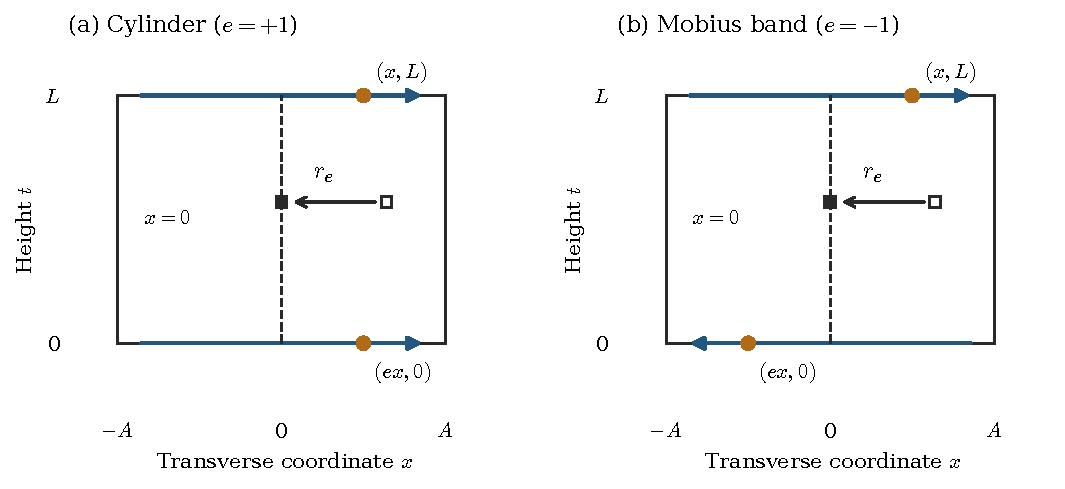
\includegraphics[width=\linewidth]{images/figure-01-quotient-seams.pdf}
\caption{Ambient cylinder and M\"obius fundamental domains. Colored circles
represent the seam equivalence $(x,L)\sim(ex,0)$; arrows encode equal or
reversed transverse orientation. Squares illustrate the central retraction
$r_e$. These are schematic ambient points, not zeta-zero measurements and
not a claim that the zero divisor descends. The dashed segment closes into
the central circle.}
\label{fig:seams}
\end{figure}

Define probability measures, for $N(H)>0$,
\begin{equation}\label{eq:empirical}
 \nu_{e,H}=\frac1{N(H)}\sum_{0<\gamma\le H}
              m_\rho\,\delta_{q_e(x_\rho,\gamma)},\qquad
 \lambda_{L,H}=\frac1{N(H)}\sum_{0<\gamma\le H}
              m_\rho\,\delta_{\{\gamma/L\}}.
\end{equation}
Write $\mu_e=(j_e)_*m_L$. On a compact metric space define
\[
 d_{\Lip}(\nu,\mu)=\sup_{\Lip(f)\le1}
      \left|\int f\dd\nu-\int f\dd\mu\right|,
\]
where tests are real-valued. Constants cancel because both masses are one.

\begin{theorem}\label{thm:limit}
For either deck sign, $\nu_{e,H}$ converges weakly to $\mu_e$,
unconditionally. More precisely,
\begin{align}
 d_{\Lip}(\nu_{e,H},\mu_e)
 &\le \frac1{N(H)}\sum_{0<\gamma\le H}m_\rho|x_\rho|
                 +L D_{1/L}^*(H) \label{eq:lipbound}\\
 &=O_L\!\left(\frac{\log\log H}{\log H}\right).\nonumber
\end{align}
The weak-limit assertion only requires Hlawka equidistribution and
\eqref{eq:density}; the displayed rate also uses \eqref{eq:fujii}.
\end{theorem}
\begin{proof}
Critical-line reflection preserves multiplicity at each positive height.
Layer cake and \eqref{eq:density}, with its uniform constant $C$, give
\begin{align*}
 \sum_{0<\gamma\le H}m_\rho|x_\rho|
 &=\int_0^{1/2}\sum_{\substack{0<\gamma\le H\\|x_\rho|>v}}
                     m_\rho\dd v\\
 &\le2CH\log H\int_0^{1/2}e^{-v\log H/4}\dd v
 \le8CH.
\end{align*}
The two-sided convention in the density input only enlarges this bound.
By \eqref{eq:retract}, replacing $f(q_e(x_\rho,\gamma))$ by
$f(j_e([\gamma]_L))$ costs at most the first term of \eqref{eq:lipbound}.
The function $g(u)=f(j_e([Lu]))$ on $[0,1]$ is periodic and $L$-Lipschitz.
It is absolutely continuous. Stieltjes integration by parts, with
$F_H(u)=\lambda_{L,H}([0,u))$, gives
\[
 \left|\int g\dd(\lambda_{L,H}-\dd u)\right|
 \le \sup_u|F_H(u)-u|\int_0^1|g'(u)|\dd u
 \le L D_{1/L}^*(H).
\]
Periodic endpoints cancel; left and right CDF conventions differ only at
atoms and have the same integral against $g'$. This proves the inequality.
Now use \eqref{eq:rvm} and \eqref{eq:fujii} for the rate.

For completeness, weak convergence for every continuous complex-valued test
does not require a transport duality theorem. Uniform continuity on $Q_e$
makes its retraction error uniformly small on $|x|<\epsilon$. The exceptional
proportion is $O(H^{-\epsilon/4})$ by \eqref{eq:density} and \eqref{eq:rvm}.
The restriction to the central circle is handled by Hlawka. Letting
$\epsilon$ decrease after taking the limit proves the claim.
\end{proof}

\begin{proposition}\label{prop:raw}
The raw positive-height pushforward
$\mathcal D_e=\sum_{\gamma>0}m_\rho\delta_{q_e(x_\rho,\gamma)}$
has infinite mass in every neighborhood of every central-circle point.
It is not locally finite and is not a Radon measure.
\end{proposition}
\begin{proof}
Such a neighborhood contains the image of a narrow transverse strip
$|x|<\delta$ above a nonempty open height arc $I$. The metric formula justifies
this statement even across the twisted seam. Through height $H$ its mass is
at least the count in \eqref{eq:arc} minus the count with $|x|\ge\delta$.
The former is $(|I|/L+o(1))N(H)$; the latter is $o(N(H))$. Their difference
diverges. A Radon measure is finite on compact sets, whereas $Q_e$ is compact
and already has infinite mass.
\end{proof}

No analogous conclusion at every off-center point is asserted: RH would
leave an off-center neighborhood with no zeros. Theorem~\ref{thm:limit}
does not say that each zero is on the central circle, only that the weighted
exceptional proportion vanishes. It therefore does not prove RH.

\section{Critical-line residue complexity}

Let $\Gamma_+$ be the distinct positive critical-line ordinates, and let
$R_L(H)$ count residues modulo $L$ represented by \emph{simple} critical-line
zeros through height $H$.

\begin{theorem}\label{thm:residue}
For every fixed $L>0$,
\begin{equation}\label{eq:residue}
 R_L(H)\ge\frac{N_0^*(H)}{\lfloor H/L\rfloor+1},\qquad
 \liminf_{H\to\infty}\frac{R_L(H)}{\log H}
        \ge\frac{0.4L}{2\pi}.
\end{equation}
In particular $\Gamma_+$ has no eventual support period.
\end{theorem}
\begin{proof}
Simple critical-line zeros have distinct ordinates. A residue class modulo
$L$ contains at most $\lfloor H/L\rfloor+1$ positive heights through $H$,
proving the first inequality. By \eqref{eq:bcy}, eventually
$N_0^*(H)\ge0.4N(H)$. Divide by $\log H$ and use
$N(H)/(H\log H)\to1/(2\pi)$ and
$(\lfloor H/L\rfloor+1)/H\to1/L$. An eventual period would leave only
finitely many residues, contradicting their unbounded number.
\end{proof}

\begin{proposition}\label{prop:closure}
Let $K_L$ be the closure in $\T_L$ of the projected positive critical-line
ordinates, or of any fixed tail of them. Then $m_L(K_L)\ge0.4$.
\end{proposition}
\begin{proof}
The all-zero height probability assigns $K_L$ at least the proportion of
simple critical-line zeros, apart from a finite prefix. Its limiting lower
mass is at least $0.4$ by \eqref{eq:bcy}. Since $K_L$ is closed, weak
convergence to Haar and the closed-set inequality imply that its Haar mass
is at least that number, explicitly
\[
 0.4\le\liminf_{H\to\infty}\lambda_{L,H}(K_L)
 \le\limsup_{H\to\infty}\lambda_{L,H}(K_L)\le m_L(K_L),
\]
identifying the unit circle with $\T_L$ by $u\mapsto[Lu]_L$.
\end{proof}
Neither this positive-measure statement nor \eqref{eq:residue} proves that
the critical-line-only sequence is equidistributed or dense. Those claims
do not follow merely by selecting a positive-proportion subsequence.

\section{Stability of the observations}\label{sec:secondary}

\begin{lemma}\label{lem:stability}
Let $D$ be a finite positive atomic measure of mass $N>0$, and $E$ another
of mass $M\ge0$. For every bounded measurable test $h$ on their common target space,
\begin{equation}\label{eq:prob-stability}
 \left|\frac{\int h\dd(D+E)}{N+M}-\frac{\int h\dd D}{N}\right|
       \le\frac{2\|h\|_\infty M}{N+M}.
\end{equation}
For a reference probability $m$ and $H>0$,
\begin{equation}\label{eq:secondary-stability}
 \left|\frac{\int h\dd E-M\int h\dd m}{H}\right|
       \le\frac{2\|h\|_\infty M}{H}.
\end{equation}
\end{lemma}
\begin{proof}
Put $A=\int h\dd D$, $B=\int h\dd E$, and $I=\int h\dd m$.
The numerator in \eqref{eq:prob-stability}, after putting it over the
denominator $N(N+M)$, is $NB-MA$. Use
$|A|\le\|h\|_\infty N$ and $|B|\le\|h\|_\infty M$.
The other inequality follows from $|B-MI|\le |B|+M|I|$.
\end{proof}

For a zero divisor $D$ define the smooth secondary functional on $\T_1$ by
\begin{equation}\label{eq:secondary}
 \mathcal S_{\alpha,H}^{D}(h)=\frac1H
 \left(\sum_{0<\gamma\le H}m_\rho h(\{\alpha\gamma\})
              -N_D(H)\int_0^1h(u)\dd u\right).
\end{equation}
Ford--Zaharescu \cite[Theorem 1 and Corollary 2]{FZ} prove for
$h\in C^2(\T_1)$ that this converges to $\int h g_\alpha$ for zeta.
For $\alpha>0$ the density is zero unless
$\alpha=r\log p/(2\pi q)$ for a prime $p$ and coprime positive integers
$r,q$. In the latter case
\begin{equation}\label{eq:bias}
 g_\alpha(u)=-\frac{\log p}{\pi}\Rea
       \sum_{k\ge1}p^{-rk/2}e^{-2\pi i qku}.
\end{equation}
The series is absolutely convergent. These are smooth-test secondary
limits, not weak convergence against every continuous test of the unbounded
signed measures, and not an established interval-indicator theorem.

\section{An infinite off-critical perturbation}\label{sec:product}

Fix $0<\eta<1/2$ and put $z_n=\eta+i2^n$ for $n\ge1$. Define
\begin{equation}\label{eq:product}
 P(w)=\prod_{n\ge1}A_n(w),\qquad
 A_n(w)=(1-w^2/z_n^2)(1-w^2/\bar z_n^2).
\end{equation}
This is a standard prescribed-divisor construction, used here as a worked
example in the setting of \cite{GX}. The exponential heights retain an $O(\log H)$ counting
perturbation; no arithmetic significance of the base two is claimed.

\begin{theorem}\label{thm:product}
The product is an even real entire function with simple zeros exactly
$\{\pm\eta\pm i2^n:n\ge1\}$. It is positive on the real and imaginary
axes. For $|w|\le R$,
\begin{equation}\label{eq:tail}
 \sum_{n>N}|A_n(w)-1|\le
 B_N(R)=\frac{2R^2}{3}4^{-N}+\frac{R^4}{15}16^{-N}.
\end{equation}
If $B_N(R)<1$, its tail factor satisfies
\begin{equation}\label{eq:tail-error}
 \left|\prod_{n>N}A_n(w)-1\right|\le\frac{B_N(R)}{1-B_N(R)}.
\end{equation}
Furthermore $\log\max_{|w|\le R}|P(w)|=O((\log(R+2))^2)$.
\end{theorem}
\begin{proof}
Because $|z_n|\ge2^n$, expansion of the paired factor gives
\[
 |A_n(w)-1|\le2R^2 4^{-n}+R^4 16^{-n}.
\]
Its compact-uniform summability proves normal convergence of the product,
hence entire holomorphy. At a point outside the prescribed zeros, the tail
has a nonzero limit by the summable-deviation infinite-product criterion;
equivalently take a sufficiently small tail and use its convergent logarithm.
Near a prescribed zero, all the other factors form a nonvanishing analytic
function. The four roots of each factor are distinct and different factors
have distinct heights. This proves the exact simple divisor.

Evenness and conjugation symmetry hold factorwise. For real $u,v$,
\[
 A_n(u)=|1-u^2/z_n^2|^2,\qquad A_n(iv)=|1+v^2/z_n^2|^2.
\]
They are positive because $z_n^2$ is nonreal. Their infinite product cannot
vanish there, by the criterion just proved, so the limit is positive.

Summing the two geometric tails gives \eqref{eq:tail}. For a finite set
of tail factors put $u_n=|A_n(w)-1|$. Expanding the product and taking
absolute values bounds its difference from one by the sum of its elementary
symmetric polynomials in the $u_n$. The degree-$k$ sum is at most
$(\sum u_n)^k$, so the difference is at most
$\sum_{k\ge1}B_N^k=B_N/(1-B_N)$. Pass to the product limit to obtain
\eqref{eq:tail-error}. This is a bound on the tail factor, even where the
finite prefix is zero; no division by that prefix is required.

Finally $|A_n(w)|\le(1+R^2 4^{-n})^2$. Split the sum of its logarithms
at $J=\lceil\log_2\max(2,R)\rceil$. The first $J$ terms are individually
$O(\log(R+2))$, and the remaining logarithms have bounded sum using
$\log(1+v)\le v$. This proves the maximum-modulus bound. In particular
$P$ has entire-function order zero.
\end{proof}

The explicit divisor and its added count are shown in Figure~\ref{fig:sparse}.

\begin{figure}[tbp]
\centering
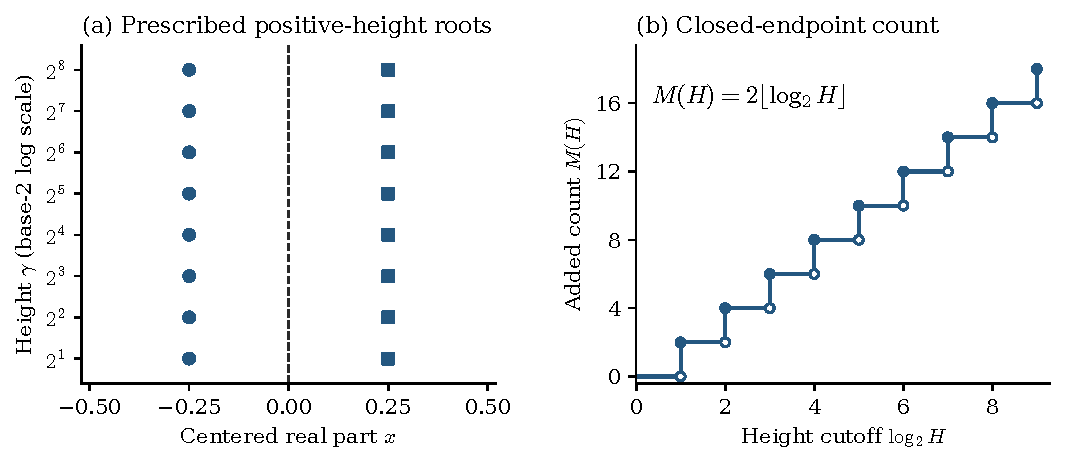
\includegraphics[width=\linewidth]{images/figure-02-sparse-divisor.pdf}
\caption{The prescribed perturbation for $\eta=1/4$, not observed zeta zeros.
Left: positive-height roots of $P$, for $1\le n\le8$, with the height axis
on a base-two logarithmic scale. Conjugate roots at negative height are
omitted. Right: the exact added count $M(H)$ through $H=2^9$; filled dots
include the dyadic endpoint and open dots show left limits. A coincidence
with a xi zero adds multiplicity rather than deleting a root.}
\label{fig:sparse}
\end{figure}

\begin{theorem}\label{thm:blindness}
Let $X(s)=\xi(s)P(s-1/2)$. It has infinitely many prescribed off-critical
zeros in the open strip, satisfies $X(1-s)=X(s)$ and the real conjugation
symmetry, and retains every critical-line zero with its original order.
Its real critical-line restriction has the same sign away from zeros.
For $H\ge2$,
\begin{equation}\label{eq:extra}
 N_X(H)=N(H)+M(H),\qquad M(H)=2\lfloor\log_2 H\rfloor.
\end{equation}
It has the same cylinder and M\"obius probability limits as zeta, and
\begin{equation}\label{eq:secondary-transfer}
 \mathcal S_{\alpha,H}^{X}(h)-\mathcal S_{\alpha,H}^{\xi}(h)\to0
\end{equation}
for every fixed $\alpha$ and bounded measurable test $h$. Consequently all
the proved smooth limits \eqref{eq:bias} persist.
\end{theorem}
\begin{proof}
Divisors of nonzero holomorphic products add, including at accidental
coincidences with xi zeros. Theorem~\ref{thm:product} inserts exactly two
positive-height roots for each $2^n\le H$, proving \eqref{eq:extra} with
the closed endpoint convention. The symmetry and sign assertions follow
from the even real structure and the positive imaginary-axis values of $P$.
Exact function values on the critical line are not preserved.
Since $M(H)=O(\log H)=o(N(H))$, \eqref{eq:prob-stability} transfers the
quotient probability limits. Inequality~\eqref{eq:secondary-stability}
bounds the difference in \eqref{eq:secondary-transfer} by
$2\|h\|_\infty M(H)/H=O(\|h\|_\infty\log H/H)$.
This transfers a limit whenever it exists; it does not establish an
unproved interval limit for either function.
\end{proof}

The Riemann--von Mangoldt main terms and its $O(\log H)$ remainder class
are unchanged. The density bound \eqref{eq:density} is unchanged as a
big-$O$ class too: the additional two-sided count is $O(\log H)$, absorbed
uniformly since $1-(\sigma-1/2)/4\ge7/8$ on the stated range.
The quotient rate is likewise unchanged in order by
\eqref{eq:prob-stability}.

Figure~\ref{fig:bounds} displays two explicit bounds used in the construction.

\begin{figure}[tbp]
\centering
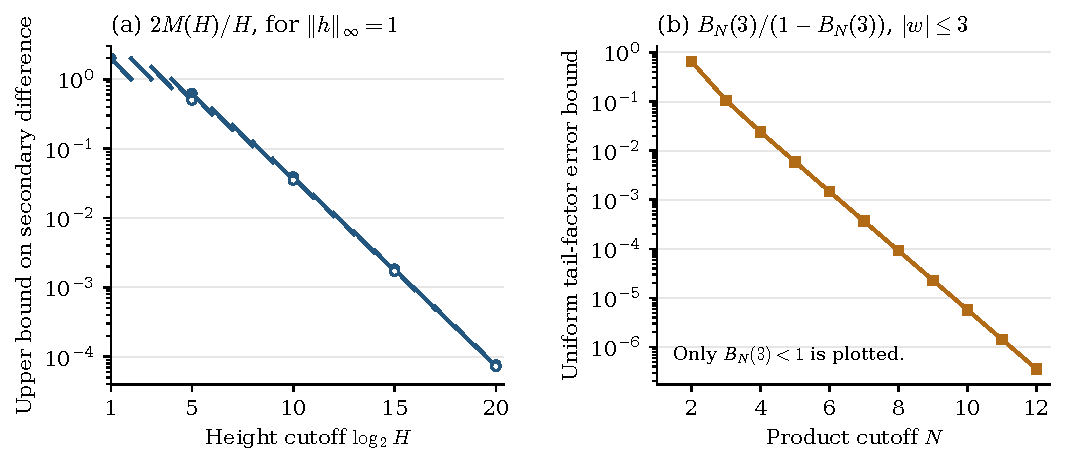
\includegraphics[width=\linewidth]{images/figure-03-certified-bounds.pdf}
\caption{Formula-based upper bounds, not measured errors. Left: the
secondary-statistic difference bound $2M(H)/H$ for
$\|h\|_\infty=1$, $2\le H\le2^{20}$; open and filled dots show selected
left limits and included endpoints. Right: the compact tail-factor bound
$B_N(3)/(1-B_N(3))$ on $|w|\le3$, plotted only when $B_N(3)<1$.
The right-hand vertical axis is logarithmic, as is the left-hand vertical
axis. Exact rational source rows and replay code accompany the figures;
the universal bounds are proved in the text.}
\label{fig:bounds}
\end{figure}

\begin{proposition}\label{prop:landau}
For every fixed $x>1$, the leading term and error class in Landau's formula
\[
 \sum_{0<\gamma\le H}m_\rho x^\rho
       =-\frac{H}{2\pi}\Lambda(x)+O_x(\log H)
\]
are preserved by $X$. Here $\Lambda(x)$ is zero unless $x$ is an integral
prime power. The error class of the uniform version in \cite[Lemma 1]{FZ}
also absorbs the perturbation for $x>1,H\ge2$.
\end{proposition}
\begin{proof}
Every added zero has real part between zero and one, so its contribution
has modulus at most $x$. The total difference is at most
$xM(H)=O(x\log H)$. For fixed $x$ this gives the first claim.
For varying $x$, the cited uniform error is
$O(x\log^2(2xH)+\log(2H)/\log x)$. Its first component absorbs this
bound. The nearest-prime-power main term is not changed.
\end{proof}
This assertion concerns asymptotic classes with unspecified constants.
It does not preserve an exact Weil explicit formula or an Euler product.
An exact added-divisor term remains present and can be detected by suitable
finite-height tests.

\section{The arithmetic boundary: an ordinary Dirichlet series}

The preceding construction can also match the pole normalization. Put
\begin{equation}\label{eq:zeta-tilde}
 \widetilde\zeta(s)=\zeta(s)\frac{P(s-1/2)}{P(1/2)}.
\end{equation}
The denominator is a strictly positive constant.

\begin{proposition}\label{prop:dirichlet}
The meromorphic function $\widetilde\zeta$ has the same gamma-factor
functional equation as zeta, the same pole at one with residue one, and
the same trivial-zero multiplicities. Nevertheless it is not representable
by any ordinary Dirichlet series absolutely convergent on a right half-plane.
\end{proposition}
\begin{proof}
The multiplier is entire, nonzero on the real axis, and invariant under
$s\mapsto1-s$. Multiplying zeta's meromorphic functional equation therefore
gives the same equation, with its usual gamma factor. Its value at $s=1$
is one, proving the residue statement. It is nonzero at each negative even
integer, so it retains every trivial-zero multiplicity.

For real $u$, direct expansion gives
\[
 A_n(u)=1+
 \frac{2(4^n-\eta^2)}{(\eta^2+4^n)^2}u^2+
 \frac{u^4}{(\eta^2+4^n)^2}\ge1.
\]
Thus $P(u)\ge A_1(u)\to\infty$ as $u\to\infty$. Since
$\zeta(\sigma)\to1$ on the positive real axis, \eqref{eq:zeta-tilde}
tends to infinity there. In contrast, if
$F(s)=\sum_{n\ge1}a_n n^{-s}$ converges absolutely at a real $\sigma_0$,
dominated convergence gives $F(\sigma)\to a_1$ as $\sigma\to\infty$:
for $\sigma\ge\sigma_0$, the summands are dominated by the summable
$|a_n|n^{-\sigma_0}$. This contradiction proves the claim.
\end{proof}

The role of an ordinary Dirichlet series is consonant with Hamburger's
converse theorem, whose precise classical formulation is recalled in
\cite[Introduction]{KMP}: if two ordinary Dirichlet series $f,g$ converge
absolutely for $\Rea s>1$, if $(s-1)f(s)$ and $(s-1)g(s)$ are entire of
finite order, and if
\[
 \pi^{-s/2}\Gamma(s/2)f(s)
 =\pi^{-(1-s)/2}\Gamma((1-s)/2)g(1-s),
\]
then $f=g=c\zeta$. We do not invoke that theorem to prove the proposition; the
positive-real-axis obstruction suffices. Extensions of converse rigidity are treated by Burnol \cite{Burnol};
related explicit non-Dirichlet functions occur in \cite{Nakamura}. The
zero-insertion literature \cite{GZ,GX} is a closer predecessor to our
construction. This proposition is an elementary check for the displayed
multiplier, not a new general nonuniqueness theorem.

\section{Verification, interpretation, and open problems}

The exact verifiers supplied with this draft check the independent geometric
tails in \eqref{eq:tail}, finite complex paired-factor and tail deviations,
prescribed roots, axis-positivity samples, dyadic count endpoints, and the
fail-closed assertion guards. Such finite arithmetic does not certify holomorphy of an
infinite product, its zero divisor, or a zeta theorem; those are the written
arguments above. The real-test algebra in Lemma~\ref{lem:stability} is
also kernel-checked in the companion \texttt{EmpiricalStability.lean} against
Lean 4.33.1 and a pinned Mathlib checkout. Its reported logical axioms are
\texttt{propext}, \texttt{Classical.choice}, and \texttt{Quot.sound}.
No claim is made of a Lean proof of the analytic input theorems or of the
whole manuscript. Earlier coordinate and zeta-support modules retain their
separate, limited coverage. The figure companion provides exact rational
source rows, vector/raster exports, independent formula checks and
regressions detecting a wrong normalization or dyadic endpoint. It uses
no empirical zeta-zero dataset.

The main conclusions distinguish three operations. An ambient height
quotient always exists. Descent of the original locally finite divisor
would require actual deck compatibility, which the support theorem excludes.
Normalized finite-height measures do converge, but their central-circle
limit and even the stated smooth secondary signatures tolerate an infinite
sparse off-critical divisor. The half-twist changes the ambient topology
without repairing these information losses.

Several questions remain meaningful. Can one obtain stronger information
about the projected critical-line-only subsequence without assuming its
equidistribution? Which \emph{exact} arithmetic identities, rather than the
asymptotic observations listed here, distinguish the zero divisor of zeta
from the sparse perturbations? How much finer a truncation-dependent test
family is needed to detect a prescribed sparse quartet? The interval
secondary asymptotics conjectured in \cite{FZ,FSZ} are not settled here.
No result in this paper proves or refutes RH.

\begin{thebibliography}{9}
\bibitem{GX}
P. M. Gauthier and X. Xarles,
\emph{Perturbations of L-functions with or without non-trivial zeros off the
critical line}, \href{https://arxiv.org/abs/0911.5135}{arXiv:0911.5135v1} (2009),
especially Proposition 1 and Theorem 2.
\bibitem{GZ}
P. M. Gauthier and E. S. Zeron,
\emph{Small Perturbations of the Riemann Zeta Function and their Zeros},
Comput. Methods Funct. Theory 4 (2004), 143--150;
\href{https://doi.org/10.1007/BF03321061}{doi:10.1007/BF03321061}.
\bibitem{Burnol}
J.-F. Burnol, \emph{Deux extensions de Th\'eor\`emes de Hamburger},
\href{https://arxiv.org/abs/1106.4749}{arXiv:1106.4749} (2011).
\bibitem{DLMF}
NIST Digital Library of Mathematical Functions,
\href{https://dlmf.nist.gov/25.4}{Section 25.4, equations 25.4.3--25.4.4}.
\bibitem{BCY}
H. M. Bui, J. B. Conrey, and M. P. Young,
\emph{More than 41\% of the zeros of the zeta function are on the critical line},
Acta Arith. 150 (2011), 35--64;
\href{https://arxiv.org/abs/1002.4127}{arXiv:1002.4127v2}.
\bibitem{FZ}
K. Ford and A. Zaharescu,
\emph{On the distribution of imaginary parts of zeros of the Riemann zeta function},
\href{https://arxiv.org/abs/math/0405459}{arXiv:math/0405459v2} (2004),
especially the Introduction, Theorem 1, Corollary 2, and Lemmas 1--2.
\bibitem{FSZ}
K. Ford, K. Soundararajan, and A. Zaharescu,
\emph{On the distribution of imaginary parts of zeros of the Riemann zeta function, II},
\href{https://arxiv.org/abs/0805.2745}{arXiv:0805.2745v3} (2009).
\bibitem{KMP}
J. Kaczorowski, G. Molteni, and A. Perelli,
\emph{A converse theorem for Dirichlet L-functions},
Comment. Math. Helv. 85 (2010), 463--483;
\href{https://sites.unimi.it/molteni/research/papers-pdf/23-molteni-A_converse_theorem_for_Dirichlet_L-functions.pdf}{author-hosted text}.
\bibitem{Nakamura}
T. Nakamura,
\emph{L-functions with the Lindel\"of and Riemann hypotheses and trivial zeros
at even negative integers}, Ann. Mat. Pura Appl. (2026),
\href{https://doi.org/10.1007/s10231-026-01726-9}{doi:10.1007/s10231-026-01726-9}.
\end{thebibliography}
\end{document}
